% Esta plantilla ha sido diseñada por Daniel del Río Velilla, profesor en la Escuela de Aeronáutica y del Espacio, UPM.
% LA PLANTILLA ES DE USO LIBRE PERO ESTÁ SUJETA A DERECHOS DE PROPIEDAD INTELECTUAL, POR LO QUE SU COMERCIALIZACIÓN ES ILEGAL.

\documentclass[11pt,a4paper,titlepage]{article}

%   ---   DEFINICION DEL TRABAJO   ---   %

\newcommand{\Project}{Motores Alternativos Aeronaúticos}
\newcommand{\ProjectTitle}{Trabajo Ciclo Termodinámico}
\newcommand{\ProjectSubject}{Grado de Ingeniería Aeroespacial}
\newcommand{\ProjectAutor}{ Cambra Valcárcel, Pablo \\
             & Del Toro Armas, Mario \\ & Gómez Jiménez, Paula\\ & Pérez Trias, Daniel\\ & Serrano Vega, Carmen}
\newcommand{\ProjectLocation}{Madrid}
\newcommand{\ProjectDate}{Diciembre 2024}
% Descomentar si se tiene un repositorio del trabajo
\newcommand{\ProjectGitHub}{url}



%   ---   INCLUIR ARCHIVOS DE CONFIGURACION   ---   %
\usepackage{chngcntr}
\counterwithin{table}{section}
\counterwithin{figure}{section} 


\usepackage[utf8]{inputenc}         % Permite escribir códigos especiales

% AJUSTES DEL IDIOMA
\usepackage[spanish]{babel}
\decimalpoint
\renewcommand{\spanishtablename}{Tabla}
\addto\extrasenglish{
    \renewcommand{\subsubsectionautorefname}{Section}
    \renewcommand{\subsectionautorefname}{Section}
    \renewcommand{\sectionautorefname}{Section}
}
\usepackage[title]{appendix}
\renewcommand{\appendixname}{Anexos}
\renewcommand{\appendixtocname}{Anexos}
\renewcommand{\appendixpagename}{Anexos}


% GEOMETRIA
\usepackage[paper=A4]{typearea}
\usepackage[includemp,
            top=2 cm,
            left = 1.2 cm, 
            right = 1.2 cm,
            bottom=2 cm,
            headsep = 3.5 cm,
            marginparwidth=2 cm,
            marginparsep=0.4 cm]{geometry}


% INDENTACION
\usepackage{indentfirst}
\setlength{\parskip}{5pt}       
\setlength{\parindent}{0pt}


% ESPACIADO
\usepackage{setspace}
\spacing{1.2}
\let\ph\mlplaceholder % shorter macro


% GENERAR PDF/A y otras cosas del pdf
\usepackage[a-1b]{pdfx}
\usepackage[pdftex]{graphicx}
    \graphicspath{
      {./Figures/Portada_HF/}
      {./Figures/01/}
      {./Figures/02/}
      {./Figures/03/}
      {./Figures/04/}
      {./Figures/05/}
      {./Figures/06/}
      {./Figures/A_01/}
      {./Figures/A_02/}
    }
\usepackage{pdfpages}               % Incluir PDF diferente tamaño


% URLS Y LINKS
\hypersetup{hidelinks}    % Hide borders links
\usepackage{url}
\Urlmuskip=0mu plus 1mu


% EXPRESIONES MATEMATICAS Y SÍMBOLOS
\usepackage{textcomp}               % Symbols in text
\usepackage{amsmath}
\usepackage{amssymb}
\usepackage{mathtools}
\usepackage[T1]{fontenc}
\usepackage{mathtools}
\usepackage{mathrsfs}
\usepackage{derivative}
\usepackage{amsmath,amssymb}
\usepackage{float}
\DeclareMathOperator{\Tr}{Tr}
\usepackage{bigints}
\usepackage{gensymb}    % Para hacer los circulitos de grados
\usepackage{eurosym}
\usepackage{fontawesome}


% INCLUIR CÓDIGO EN EL DOCUMENTO
\usepackage{listings}
\renewcommand{\lstlistingname}{Listado}		% Para que las listas sean es español
\usepackage[framed,numbered,autolinebreaks,useliterate]{mcode}      % MATLAB CODE
% \lstset{
%     inputencoding=utf8,
%     literate={Á}{{\'A}}1 {á}{{\'a}}1 {É}{{\'E}}1 {é}{{\'e}}1 {Í}{{\'I}}1 {í}{{\'i}}1 {Ó}{{\'O}}1 {ó}{{\'o}}1 {Ú}{{\'U}}1 {ú}{{\'u}}1 
%     }

%\lstset{
%  basicstyle         = \mlttfamily,
%  escapechar         = ",
%}
%\usepackage[numbered]{matlab-prettifier}


% ACRONIMOS
% https://tex.stackexchange.com/questions/25520/how-can-i-use-the-latex-acronym-package-and-optionally-create-an-acronym-list-i
% https://sourceforge.net/p/texstudio/discussion/907839/thread/7ced058c/  -> SI NO APARECEN LOS ACRONIMOS
\usepackage[acronym,smallcaps]{glossaries}[=v4.46]		% ,nonumberlist
% \loadglsentries[\acronymtype]{./Tex_Files/acronyms.tex}
\makeglossaries
%\usepackage{nomencl}
%\makenomenclature
%\usepackage{etoolbox}
%\renewcommand\nomgroup[1]{%
%  \item[\bfseries
%  \ifstrequal{#1}{P}{Propiedades físicas}{%
%  \ifstrequal{#1}{S}{Señales ópticas}{%
%  \ifstrequal{#1}{F}{Fibra óptica}{%
%  \ifstrequal{#1}{C}{Material compuesto}{}}}}%
% ]}


% BIBLIOGRAFÍA
%\usepackage{biblatex}
%\addbibresource{references.bib}
%\setlength\parindent{0pt}


% DISEÑO DE TABLAS Y FIGURAS 
% \usepackage{subfigure}
% \usepackage{subfloat}
\usepackage{caption}
\usepackage{subcaption}		% https://tex.stackexchange.com/questions/295456/texstudio-beginsubfigure-unrecognized-command
\usepackage{svg}
\usepackage{import}
\usepackage{longtable}
\usepackage{multirow}
\usepackage{multicol}
\usepackage{threeparttable}
\usepackage{booktabs}
\usepackage{tabu}
\usepackage{bigstrut}
\usepackage{tabularx}
    \makeatletter
    \def\hlinewd#1{%
    \noalign{\ifnum0=`}\fi\hrule \@height #1 \futurelet
    \reserved@a\@xhline}
    \makeatother
\usepackage{placeins}  %para poder poner Floatbarrier


% ENUMERACIONES
\usepackage{enumerate}
\usepackage{enumitem}  % Selecionar la forma del item


% NOTAS PIE DE PAGINA
\usepackage[colorinlistoftodos]{todonotes}  % TO DO
\newcommand\blfootnote[1]{%
  \begingroup
  \renewcommand\thefootnote{}\footnote{#1}%
  \addtocounter{footnote}{-1}%
  \endgroup
}


% DEFINICIÓN DE COLORES 
\usepackage{xcolor}
\usepackage{colortbl}


% COMANDOS
\providecommand\phantomsection{}    % Para añadir phantomsections al indice


% LANDSCAPE
\usepackage{pdflscape}
\usepackage{everypage}
\usepackage{lipsum}
% Landscape configuration
\newcommand{\Lpagenumber}{\ifdim\textwidth=\linewidth\else\bgroup
  \dimendef\margin=0 %use \margin instead of \dimen0
  \ifodd\value{page}\margin=\oddsidemargin
  \else\margin=\evensidemargin
  \fi
  \raisebox{\dimexpr -\topmargin-\headheight-\headsep-0.5\linewidth}[0pt][0pt]{%
    \rlap{\hspace{\dimexpr \margin+\textheight+\footskip}}}%
\egroup\fi}
\AddEverypageHook{\Lpagenumber}%
% Code
%\begin{landscape}
% Text
%\end{landscape}


% MISCELANEO
\usepackage{cite}
\usepackage{csquotes} % Cita en el texto
\usepackage{comment} % Comentar en bloque
\usepackage{lastpage} % Citar la última página
\usepackage{relsize} % Tamaños relativos
\usepackage{bm} % Para poner negrita math tablas
\usepackage{printlen}
\usepackage{afterpage}	% añadir algo despues de una pagina
\newacronym{mc}{MC}{Materiales Compuestos}
\newacronym{cfrp}{CFRP}{Carbon Fiber Reinforced Polymer}
\newacronym{udpp}{UDPP}{Unidirectional Prepeg}
\newacronym{fr}{FR}{Filament Ripper}
\newacronym{rrf}{RRF}{RepRap Firmware}
\newacronym{dwc}{DWC}{Duet Web Control}
\newacronym{sbc}{SBC}{Single Board Computer}
\newacronym{rsp}{RSP4}{Raspberry Pi 4}
\newacronym{cad}{CAD}{Computer Aided Desing}
\newacronym{rpas}{RPAS}{Remotely Piloted Aircraft System}
\newacronym{ba}{BA}{Borde de ataque}
\newacronym{bs}{BS}{Borde de salida}
\newacronym{eop}{EoP}{Edge of Part}
\newacronym{eeop}{EEoP}{Engineering Edge of Part}
\newacronym{meop}{MEoP}{Manufacturing Edge of Part}
\newacronym{eom}{EoM}{Excess of Material}
% DISEÑO DE CABECERA Y PIE DE PÁGINA
\lstMakeShortInline"
\newlength{\myoddoffset}
\setlength{\myoddoffset}{\marginparwidth + \marginparsep + 0.5cm}
\usepackage{fancyhdr}
\fancyheadoffset[rh]{\myoddoffset}
\fancyfootoffset[rh]{\myoddoffset}

\pagestyle{fancy}
\fancyhf{}
\fancyhead[R]{ \hspace{2pt} \rightmark}
\lhead{
    
\includegraphics[width = 4.2cm]{upm_logo.png}
}
\rhead{
    \begin{Large}{\Project}\end{Large}
}
% \lfoot{} \cfoot{} \rfoot{\thepage}
\fancyfoot[RO]{\thepage}


\newgeometry{
    top=1.7in, 
    bottom=1.1in, 
    left = 2.5cm, 
    right = 2cm, 
    headsep = 2.5cm, 
    ignoremp
}
\fancyheadoffset[rh]{0pt}
\fancyfootoffset[rh]{0pt}

\fancypagestyle{plain}{		% Modificar el pagenumber en los capitulos
	\fancyhf{} 
	\fancyfoot[RO]{\thepage} % same placement as with page style "fancy"
	\renewcommand{\headrulewidth}{0pt}
	}
	


% % ABSTRACT
% \def\changemargin#1#2{\list{}{\rightmargin#2\leftmargin#1}\item[]}
% \let\endchangemargin=\endlist 
% \newcommand\summaryname{Abstract}
% \newenvironment{Abstract}%
%     {\small\begin{center}%
%     \bfseries{\summaryname} \end{center}}
\newcommand{\clearemptydoublepage}{
    \newpage{\pagestyle{empty}\cleardoublepage}
}

\newcommand\blankpage{%
    \null
    \thispagestyle{empty}%
    \addtocounter{page}{-1}%
    \newpage}



%   ---   COMIENZO DEL DOCUMENTO   ---   %

\begin{document}


%   ---   INCLUIR PORTADA   ---   %

\begin{titlepage}
	\begin{center}
		\vspace*{0in}
		\begin{figure}[htb]
			\centering
			\includegraphics[width = 0.6\linewidth]{./Figures/Portada_HF/UPM_logo.png}
		\end{figure}
		
		\vspace*{0.2in}
		\rule{\linewidth}{0.4mm}\\
		\vspace*{0.1in}
		\begin{huge}
			\textbf{\scshape{\ProjectTitle}} \\
		\end{huge}
		\vspace*{0.1in}
		\begin{large}
			\begin{normalsize}
				\scshape{\Project}\\
				\scshape{\ProjectSubject}
			\end{normalsize}
		\end{large} 
		\vspace*{0.2in}
		\rule{\linewidth}{0.4mm}\\
		\vspace*{0.6in}
		\begin{large}
			\begin{tabular}{c}
				\\
				\begin{tabular}{ l l }
					\textit{Autores}: & \ProjectAutor     \\
					                &                   \\
					%\textit{Tutor}: & \ProjectTutor     \\
					 %               &                   \\
				\end{tabular}
				
				
			\end{tabular}
		\end{large}
		
		\vspace*{0.5in}
		\begin{large}
			\textsc{\ProjectLocation, \ProjectDate}
		\end{large}
	\end{center}
	
	% Repositorio: descomentar si se usa un repo
	% \begin{center}
		% \vspace*{\fill}\begin{LARGE}\faGithub\end{LARGE}\hspace{2mm}\url{\ProjectGitHub}
	% \end{center}
	
\end{titlepage}




%   ---   INDICE Y LISTAS   ---   %

% Indice
\pagenumbering{gobble}
\tableofcontents
\newpage

% Numeracion en romano
\pagenumbering{roman}
\raggedbottom

% Figuras    
\addcontentsline{toc}{section}{\listfigurename}
\listoffigures
\clearpage

% Tablas
\renewcommand{\listtablename}{Índice de tablas}
\addcontentsline{toc}{section}{\listtablename}
\listoftables
\clearpage


% Numeracion en arabico
\setcounter{page}{0}
\pagenumbering{arabic}



%   ---   ARCHIVOS DEL DOCUMENTO   ---   %
% Es recomendable escribir el trabajo en documentos separados y luego importarlos al main.

\section{Potencia y Cilindrada} \label{s:section_01}

Para este trabajo se estudiará un motor de competición para un BMW M4 GT3. Se busca que pase de 0 a 100 km/h en tiempos próximos a 2 segundos y alcance velocidades máximas cercanas a 250 km/h. 

Para determinar la potencia que debe producir el motor, se cuentan con los siguientes datos:

\begin{itemize}
    \item \textbf{Masa del coche:} Entre 1 y 1.5 toneladas.
    \item \textbf{Corte de inyección:} 9000 rpm.
    \item \textbf{Pérdidas en la transmisión:} 15\% de la potencia al freno.
    \item \textbf{Coeficiente de resistencia aerodinámica (\(C_d\)):} 0.40.
    \item \textbf{Área frontal:} 3.0 m².
    \item \textbf{Momento de inercia global:} \( 0.3 \, \text{kg}\text{m}^2 \).
\end{itemize}

Para garantizar un enfoque conservador, se han seleccionado los datos que conducen a las condiciones más exigentes.

El cálculo de la potencia necesaria para el motor considera las siguientes contribuciones de potencia:

\begin{equation}
\dot{W}_{\text{motor}} = \dot{W}_{\text{aero}} + \dot{W}_{\Delta Ep} + \frac{d}{dt} \left[ \frac{1}{2} m v^2 \right] + \frac{1}{2} \sum_{i} I_i \omega_i^2
\end{equation}

\subsection*{Cálculo de términos}

El primer término representa la potencia disipada por la resistencia aerodinámica al ir a 100 km/h:
\[
\dot{W}_{\text{aero}} =  \frac{1}{2}  \rho_a  C_d  A_fv^3 = 16 \, \text{kW}
\]

El segundo término representa la potencia asociada al cambio de energía potencial asumiendo una inclinación del 17\% (Eau Rouge-Radillon en Spa-Francorchamps) : 
\[
\dot{W}_{\Delta Ep} = \frac{\Delta Ep}{\Delta t} = 125 \, \text{kW}
\]

El tercer término representa la potencia asociada a acelerar el vehículo (de 0 a 100 km/h en 2 segundos): % de 0 a 100 en 2 segundos
\[
\frac{d}{dt} \left[ \frac{1}{2} m v^2 \right] =\frac{1}{2}  m  \frac{v_f^2 - v_i^2}{t} = 289 \, \text{kW}
\]
El cuarto término representa la potencia asociada a acelerar las partes móviles del vehículo (de 0 a 100 km/h en 2 segundos):
\[
\frac{1}{2} \sum_{i} I_i \omega_i^2 = \frac{1}{2} \  I_g \  \frac{\omega_f^2 - \omega_i^2}{t} = 67 \, \text{kW}
\]

Por tanto, la potencia total del motor será: \\
\[
\dot{W}_{\text{motor}} = 497 \, \text{kW}
\]

\section{Carrera y Cilindrada} \label{s:section_02}

El motor seleccionado tiene una cilindrada de 3 litros y cuenta con 6 cilindros en línea, con la idea de que sea lo más similar posible a uno de los motores habitualmente instalado por BMW en sus M3 (antecesores al M4).

En la figura \ref{fig:RPM_sb}, se observa la relación entre las revoluciones por minuto (\textit{rpm}) y la potencia del motor. Se ha elegido la curva más lineal (aquella que corresponde a un motor más \textit{elástico}), correspondiente a la carrera de 62 \text{mm}.

\begin{figure}[H]
    \centering
    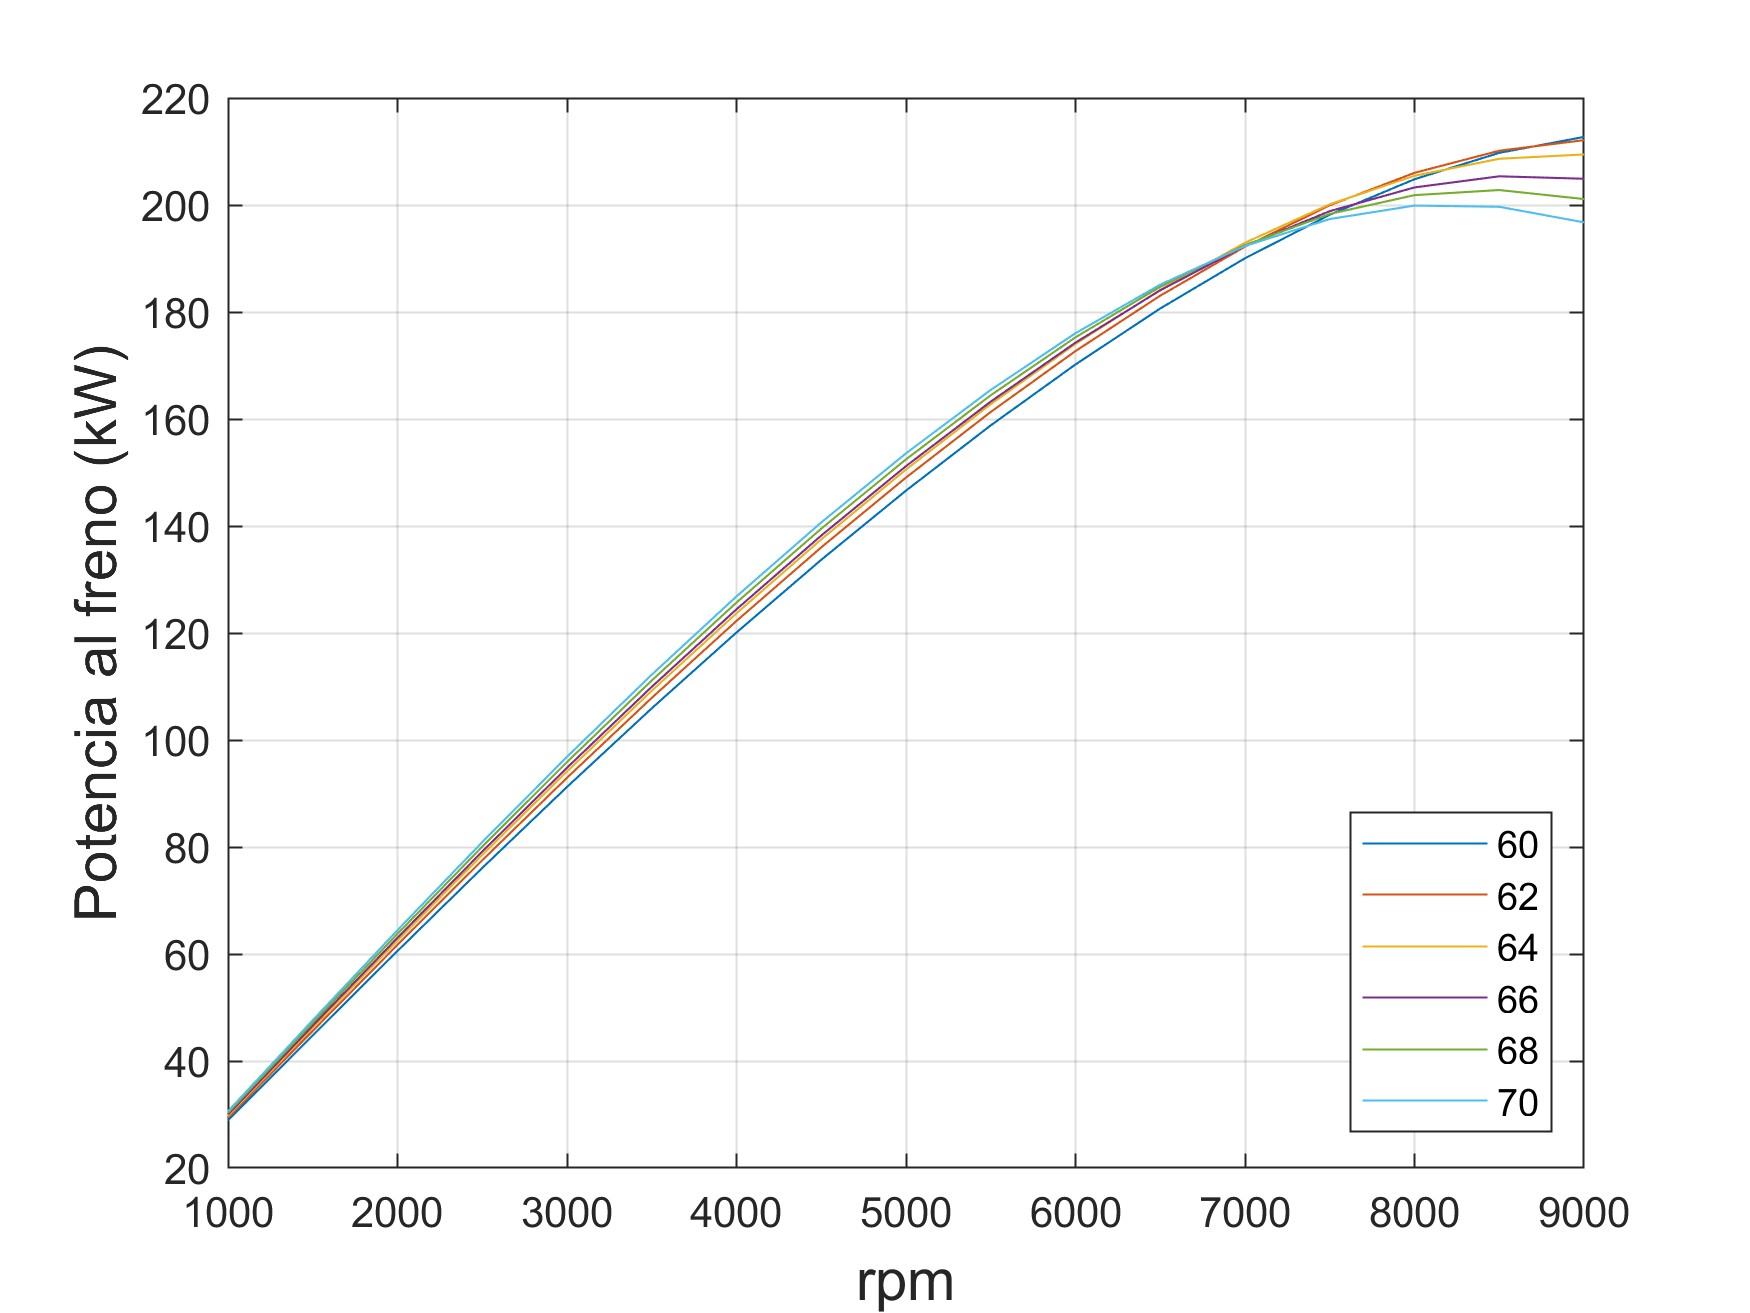
\includegraphics[width=0.6\linewidth]{Figures/01/Potencia_rpm_sb.jpg}
    \caption{Potencia en función de las rpm para cada carrera.}
    \label{fig:RPM_sb}
\end{figure}

La curva de potencia elegida para el estudio se corresponde con una carrera \( s = 62 \, \text{mm} \) y con un radio del émbolo \( b = 101 \, \text{mm} \).

\section{Retardo al Cierre de Admisión} \label{s:section_03}
Para determinar el retardo del cierre de la válvula de admisión se ha ejecutado un bucle que proporciona las curvas de potencia al freno del motor para distintos valores de dicho ángulo. Una vez obtenida esa gráfica (figura \ref{fig:RPM_rca}) se escoge, para cada intervalo de revoluciones, el valor que mayor potencia proporciona. Esos valores se recogen en la tabla \ref{tab:rpm_RCA}, y a partir de ellos se genera un polinomio de orden 3 (implementado a posteriori en una función) de manera que, para un valor arbitrario de revoluciones del motor, se recibe (redondeado al entero más próximo) el valor óptimo de este parámetro. Los resultados de este polinomio y los datos contenidos en la tabla se observan en la figura \ref{fig:RPM_rca_regresión}.

\begin{figure}[H]
    \centering
    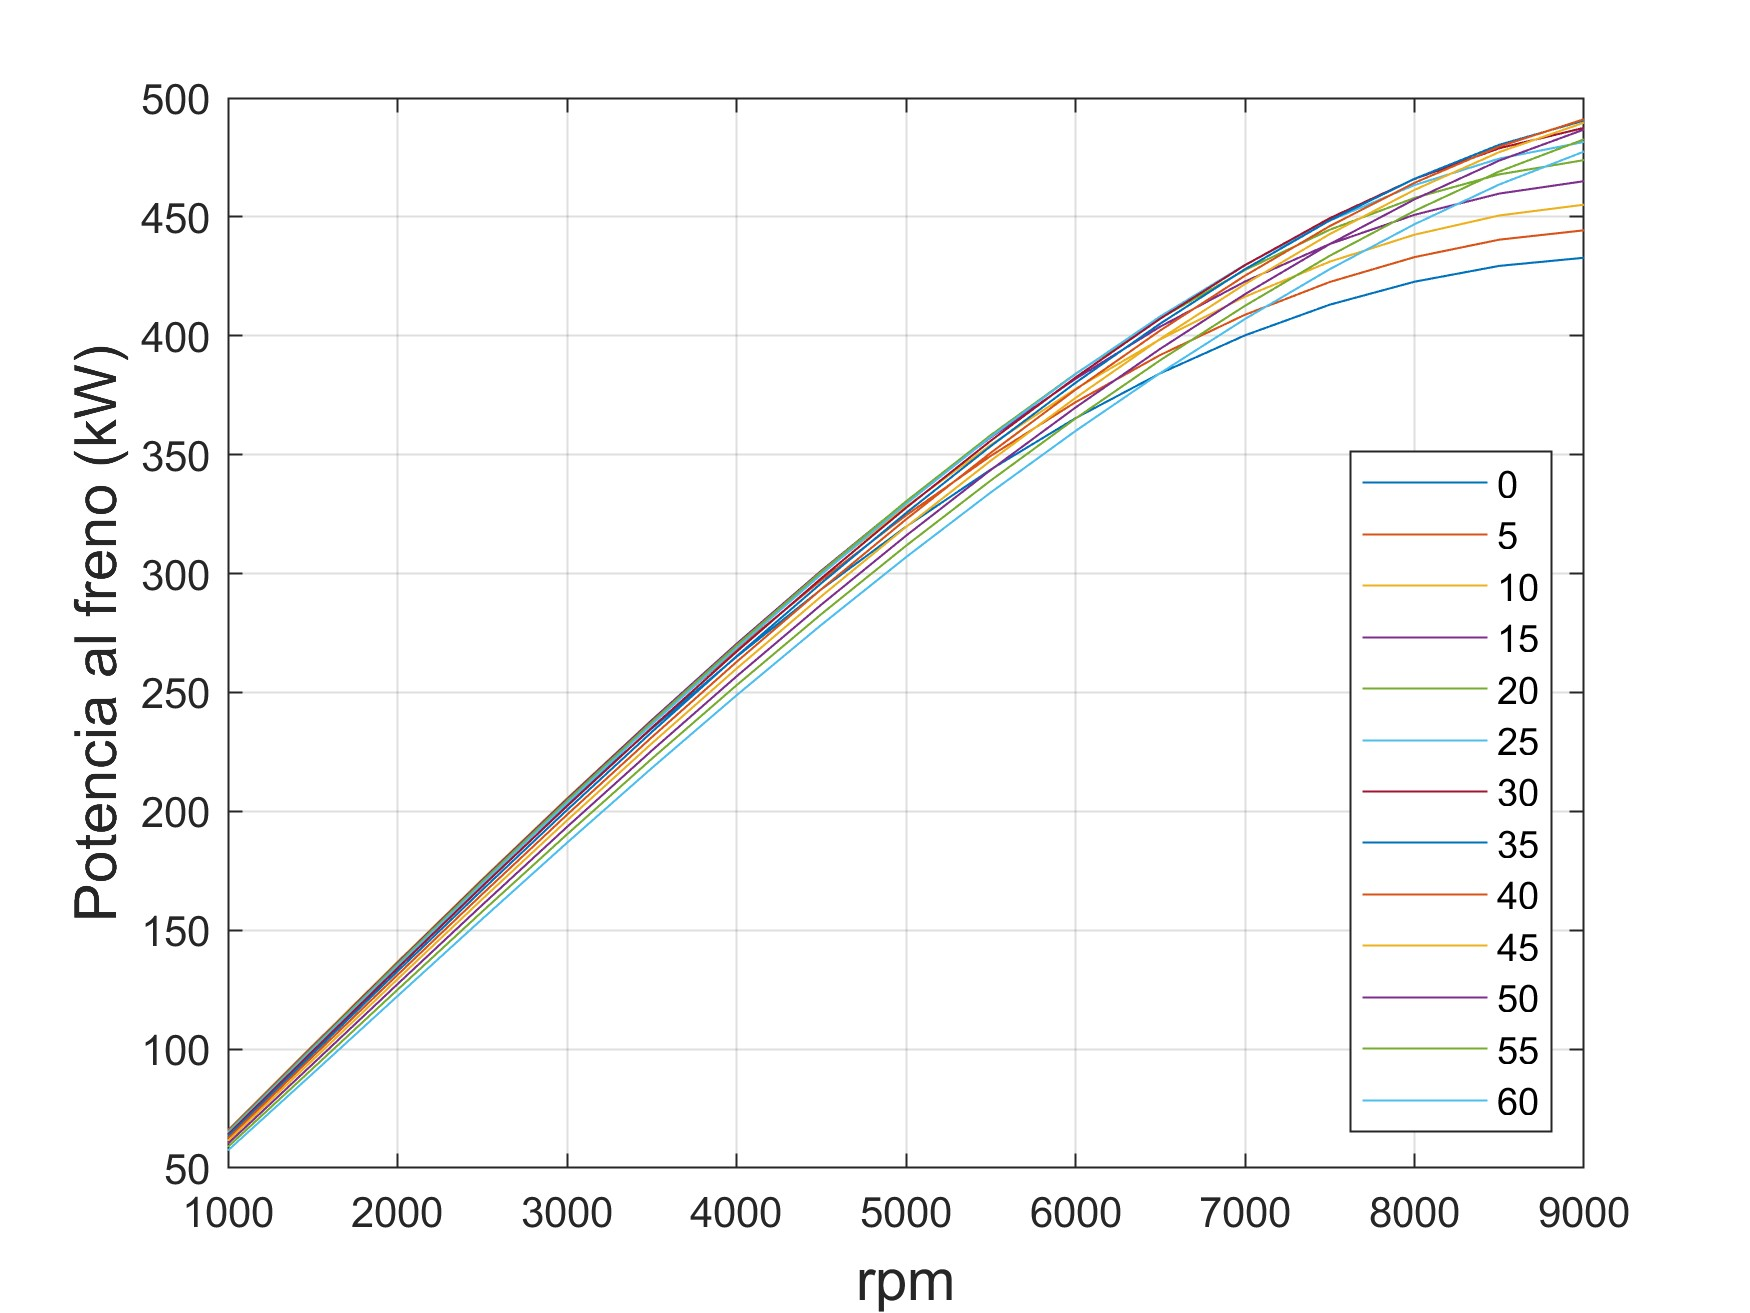
\includegraphics[width=0.6\linewidth]{Figures/01/Potencia_rpm_rca.jpg}
    \caption{Potencia en función de las rpm para cada retardo al cierre de admisión.}
    \label{fig:RPM_rca}
\end{figure}

\begin{table}[htbp]
    \centering
    \resizebox{1\textwidth}{!}{
        \begin{tabular}{|c|*{8}{c|}}
           \hline 
           \textbf{rpm} & 0-2000 & 2000-3500 & 3500-4800 & 4800-6000 & 6000-6900 & 6900-7750 & 7750-8500 & 8500-9000 \\
           \hline 
           RCA [°] & 5 & 10 & 15 & 20 & 30 & 35 & 40 & 45 \\
           \hline
        \end{tabular}
    }
    \caption{Retardos de cierre de admisión que obtienen mayor potencia en función de las rpm.}
    \label{tab:rpm_RCA}
\end{table}

\begin{figure}[H]
    \centering
    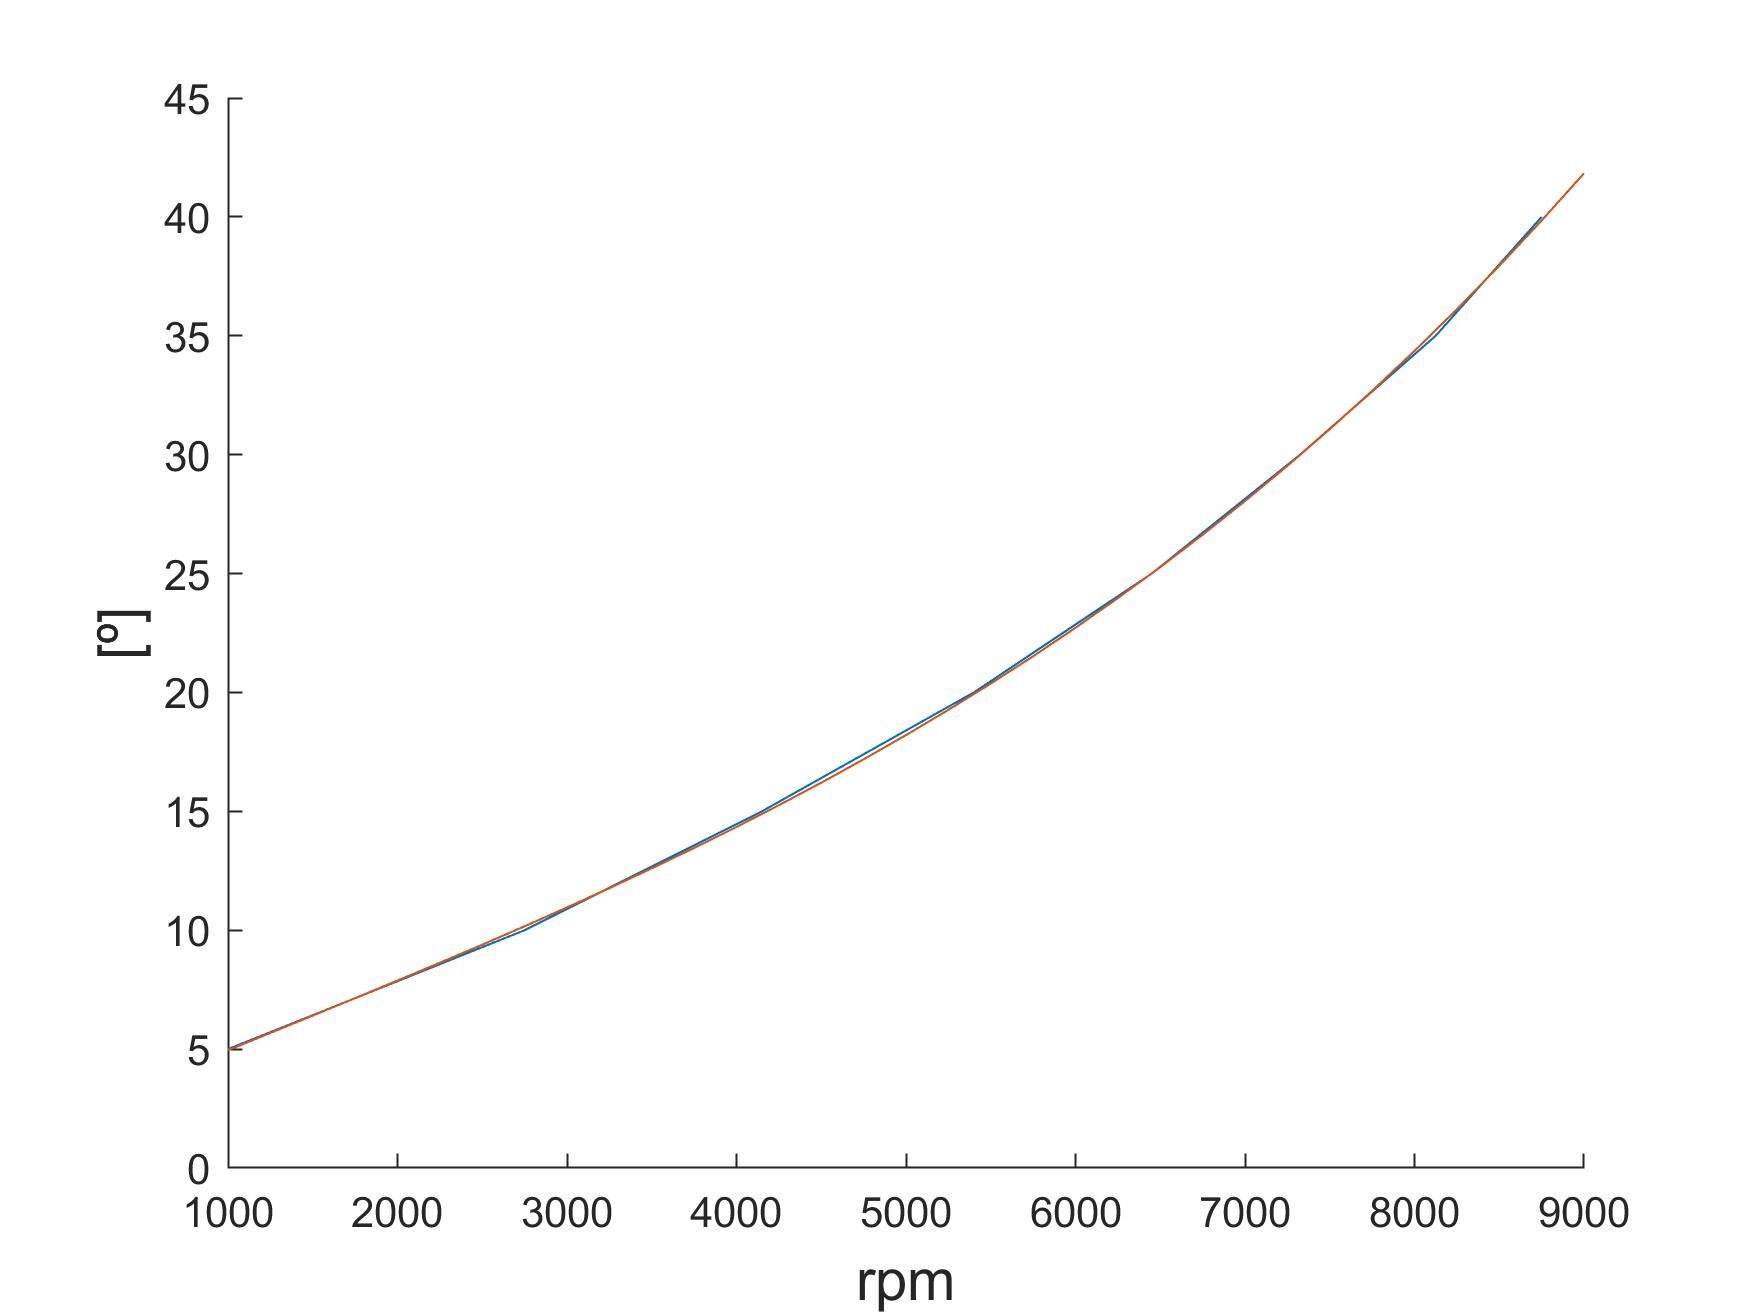
\includegraphics[width=0.6\linewidth]{Figures/01/regresion_rca.jpg}
    \caption{Polinomio del retardo al cierre de admisión en función de las rpm.}
    \label{fig:RPM_rca_regresión}
\end{figure}







\section{Adelanto a la apertura de escape} \label{s:section_04}

Se procede de forma análoga al apartado anterior y se recoge la potencia al freno del motor para distintos valores de dicho ángulo \ref{fig:RPM_aae}. A través de esta gráfica se obtiene la tabla \ref{tab:rpm_AAE}. Los resultados de realizar una regresión igual a la utilizada con el RCA y los datos contenidos en la tabla se observan en la figura \ref{fig:RPM_aae_regresión}.

\begin{figure}[H]
    \centering
    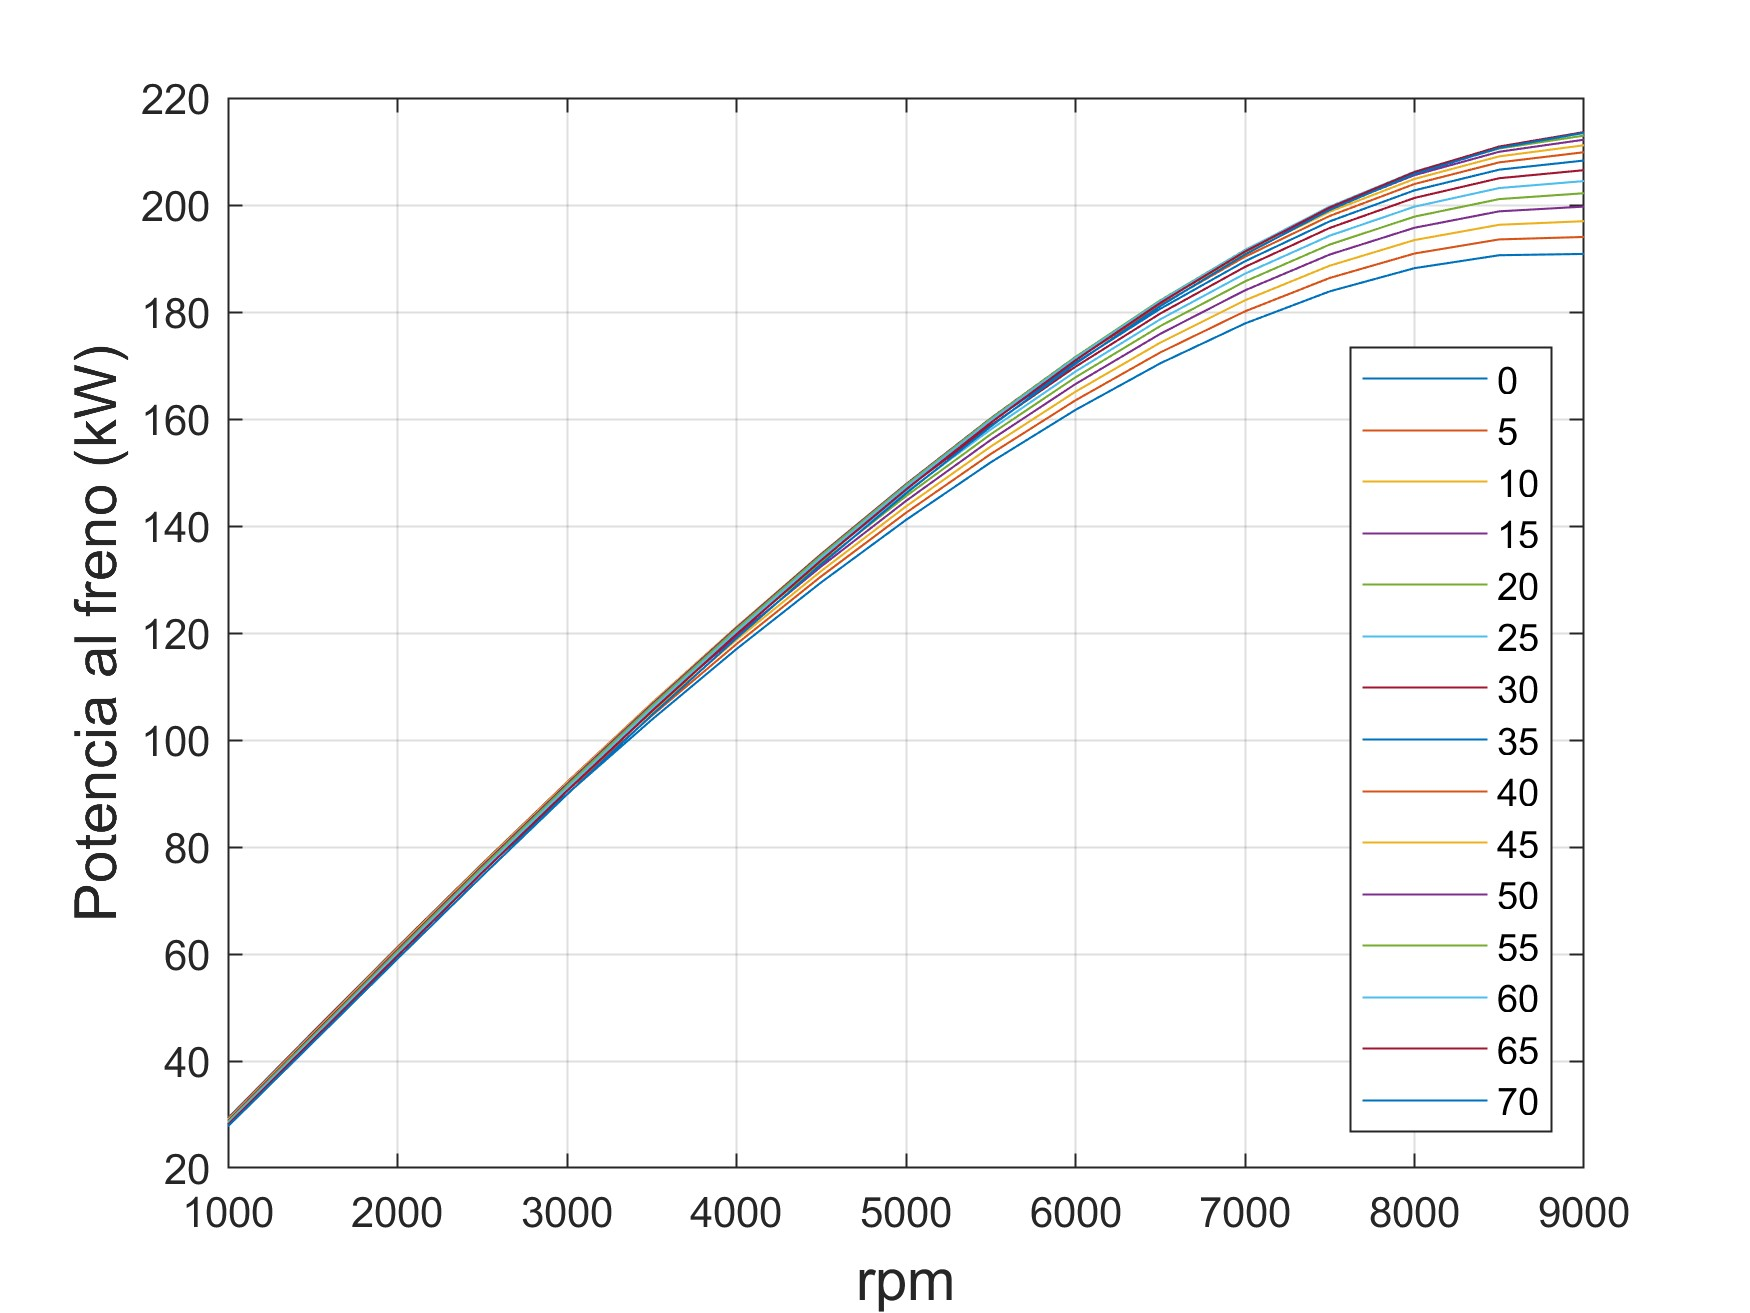
\includegraphics[width=0.6\linewidth]{Figures/01/Potencia_rpm_aae.jpg}
    \caption{Potencia en función de las rpm para cada adelanto a la apertura de escape.}
    \label{fig:RPM_aae}
\end{figure}

\begin{table}[htbp]
    \centering
    \resizebox{1\textwidth}{!}{
        \begin{tabular}{|c|*{9}{c|}}
           \hline 
           \textbf{rpm} & 0-1750 & 1750-2500 & 2500-3250 & 3250-4000 & 4000-5000 & 5000-6000 & 6000-7000 & 7000-8500 & 8500-9000 \\
           \hline 
           RCA [°] & 30 & 35 & 40 & 45 & 50 & 55 & 60 & 60 & 65 \\
           \hline
        \end{tabular}
    }
    \caption{Adelantos de apertura de escape que obtienen mayor potencia en función de las rpm.}
    \label{tab:rpm_AAE}
\end{table}

\begin{figure}[H]
    \centering
    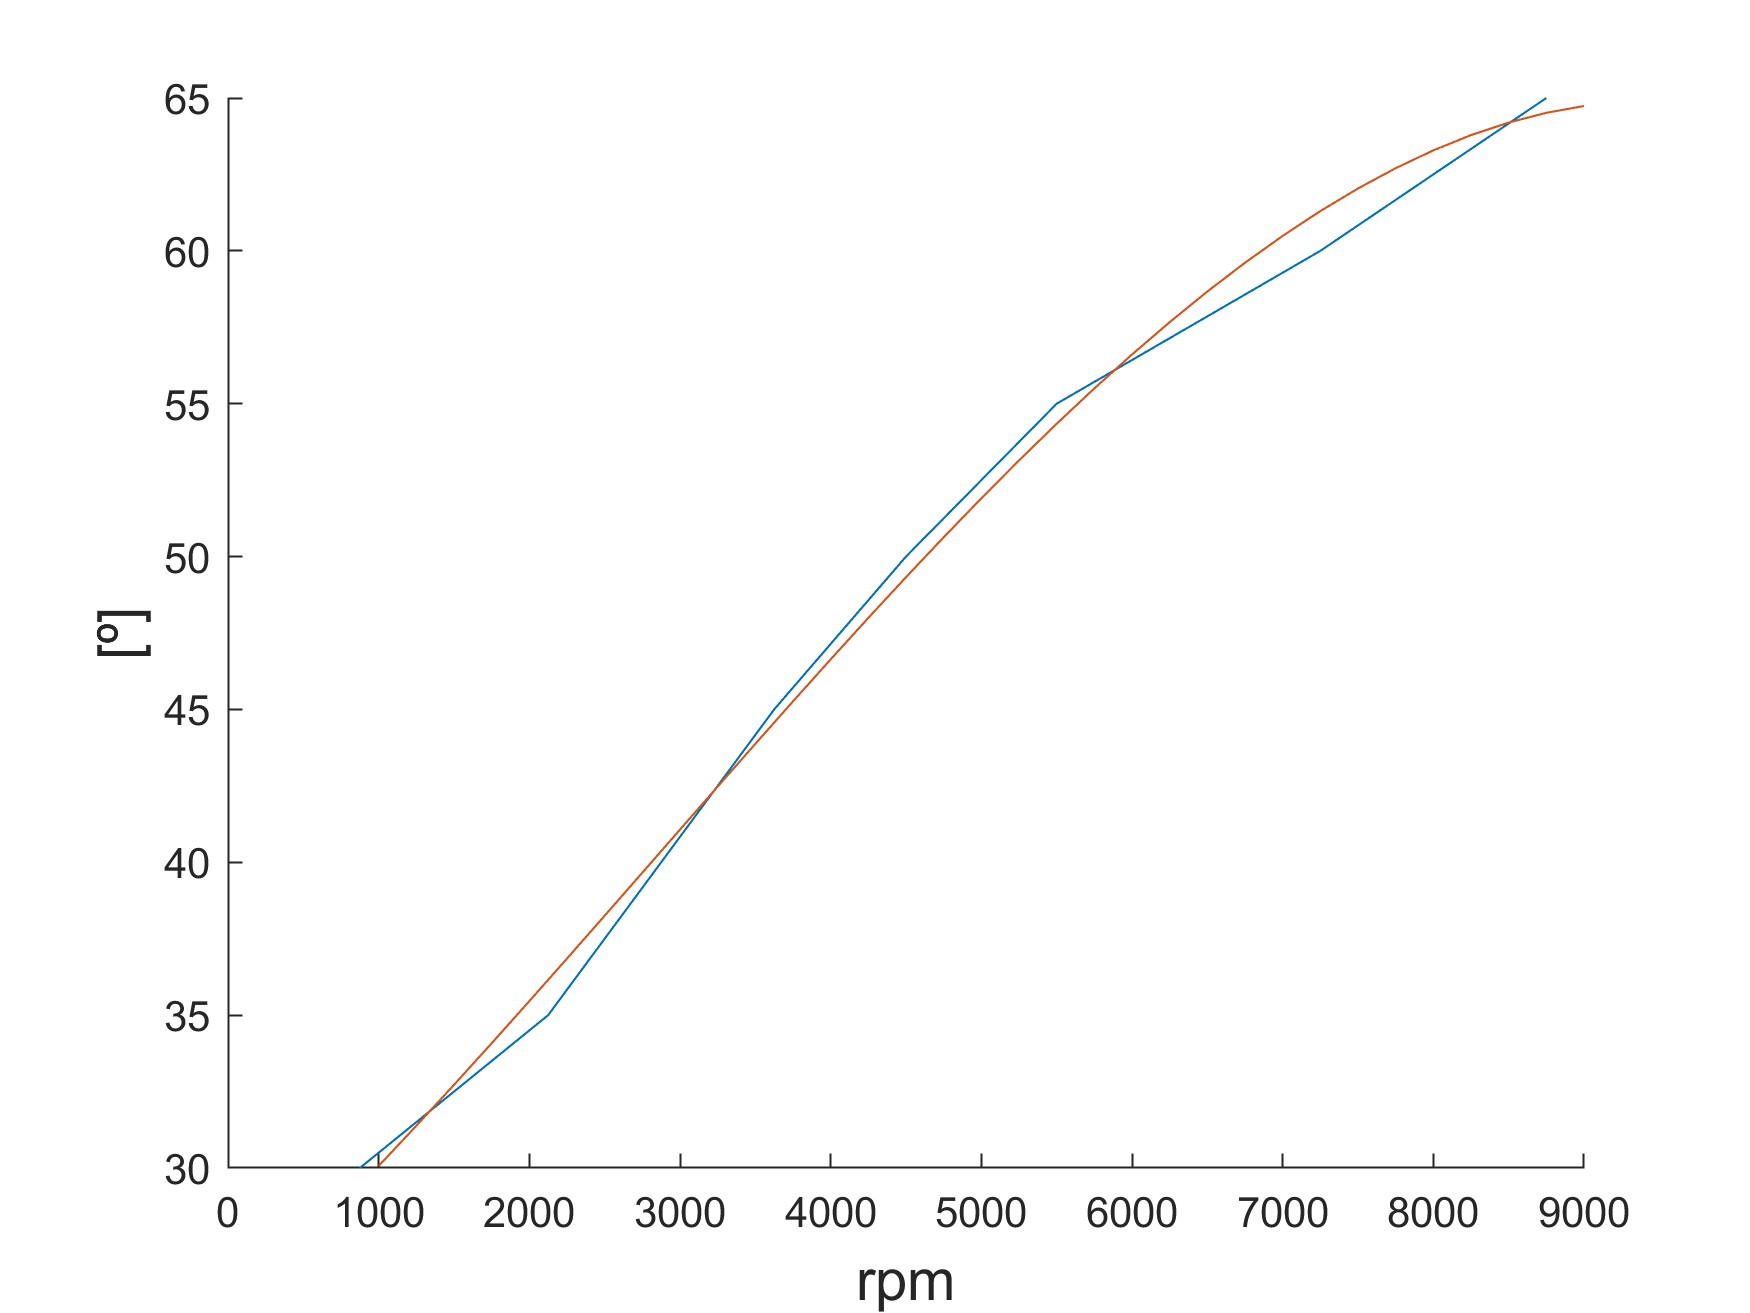
\includegraphics[width=0.6\linewidth]{Figures/01/regresion_aae.jpg}
    \caption{Polinomio del adelanto de apertura de escape en función de las rpm.}
    \label{fig:RPM_aae_regresión}
\end{figure}



\section{Elección de los Parámetros} \label{s:section_05}
\subsection{Relación de Compresión Geométrica} \label{s:subsection_01}
Inicialmente se empleó una relación de compresión de 7.5, al ver que este se podía subir sin generar problemas de detonación que no se pudiesen solucionar modificando los ángulos de ignición, se decidió subir a 9.5. A su vez, al haber elegido un vehículo deportivo turboalimentado, en la modelización de este se considera una presión de admisión algo mayor que la correspondiente con la ambiente al nivel del mar; es decir, alrededor de 2 bares; mientras que la presión de escape será el 80\% de esta última.

\subsection{Áreas de válvulas} \label{s:subsection_02}
\begin{itemize}
   \item \textbf{Área de válvula de admisión (AA):} 33\%  del área del cilindro.
  \item \textbf{Área de válvula de escape (AE):} 28\%  del área del cilindro.
  \end{itemize}

A partir de esta configuración inicial, se evalúa el impacto de variaciones, en este caso, aumento; en el tamaño del área efectiva de las válvulas sobre el rendimiento del motor.

\begin{figure}[H]
    \centering
    % Subfigura 1
    \begin{subfigure}[b]{0.45\textwidth}
        \centering
        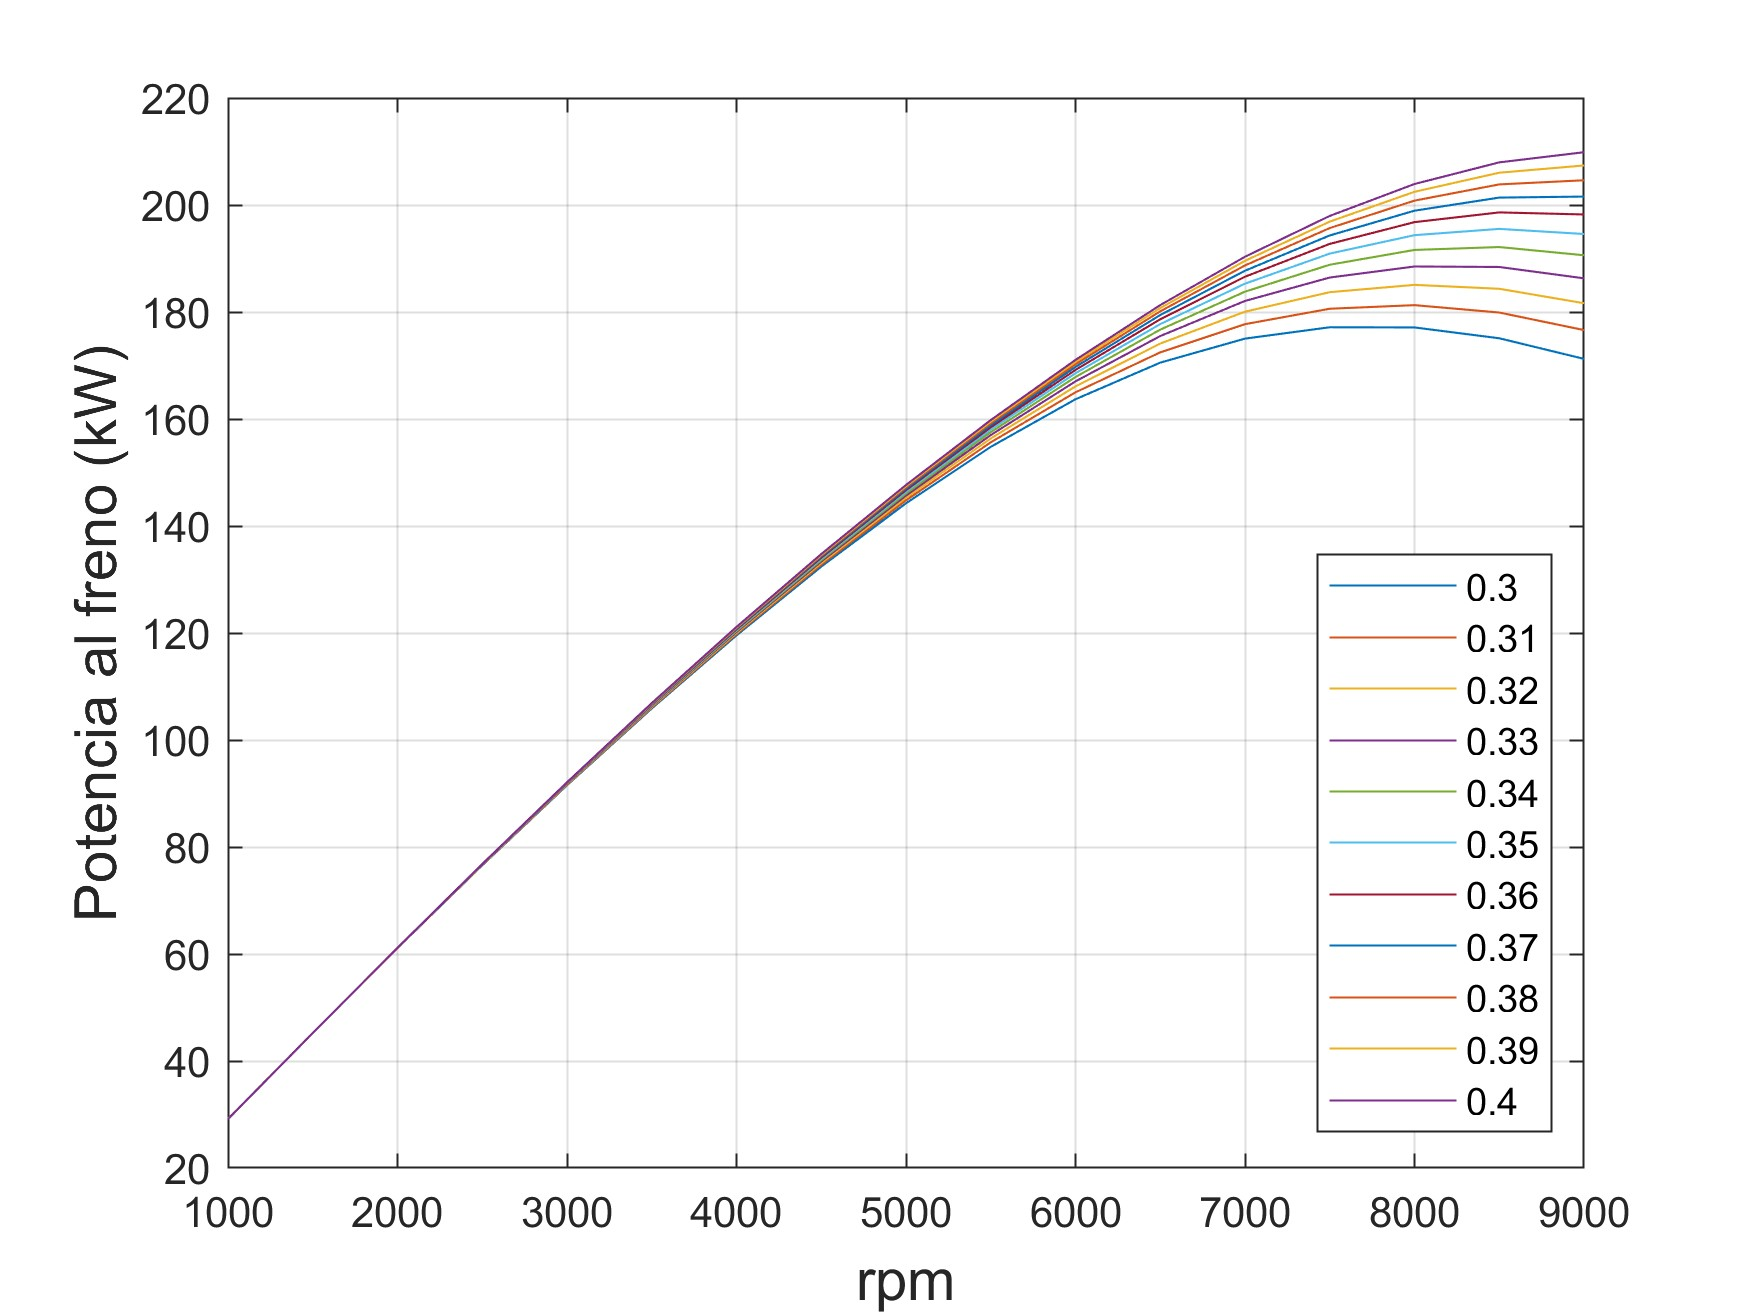
\includegraphics[width=\linewidth]{Figures/01/Potencia_rpm_aval_admision.jpg}
        \caption{Potencia en función de las rpm para dicha área de válvula de admisión (AA).}
        \label{fig:RPM_aval_admision}
    \end{subfigure}
    \hfill
    % Subfigura 2
    \begin{subfigure}[b]{0.45\textwidth}
        \centering
        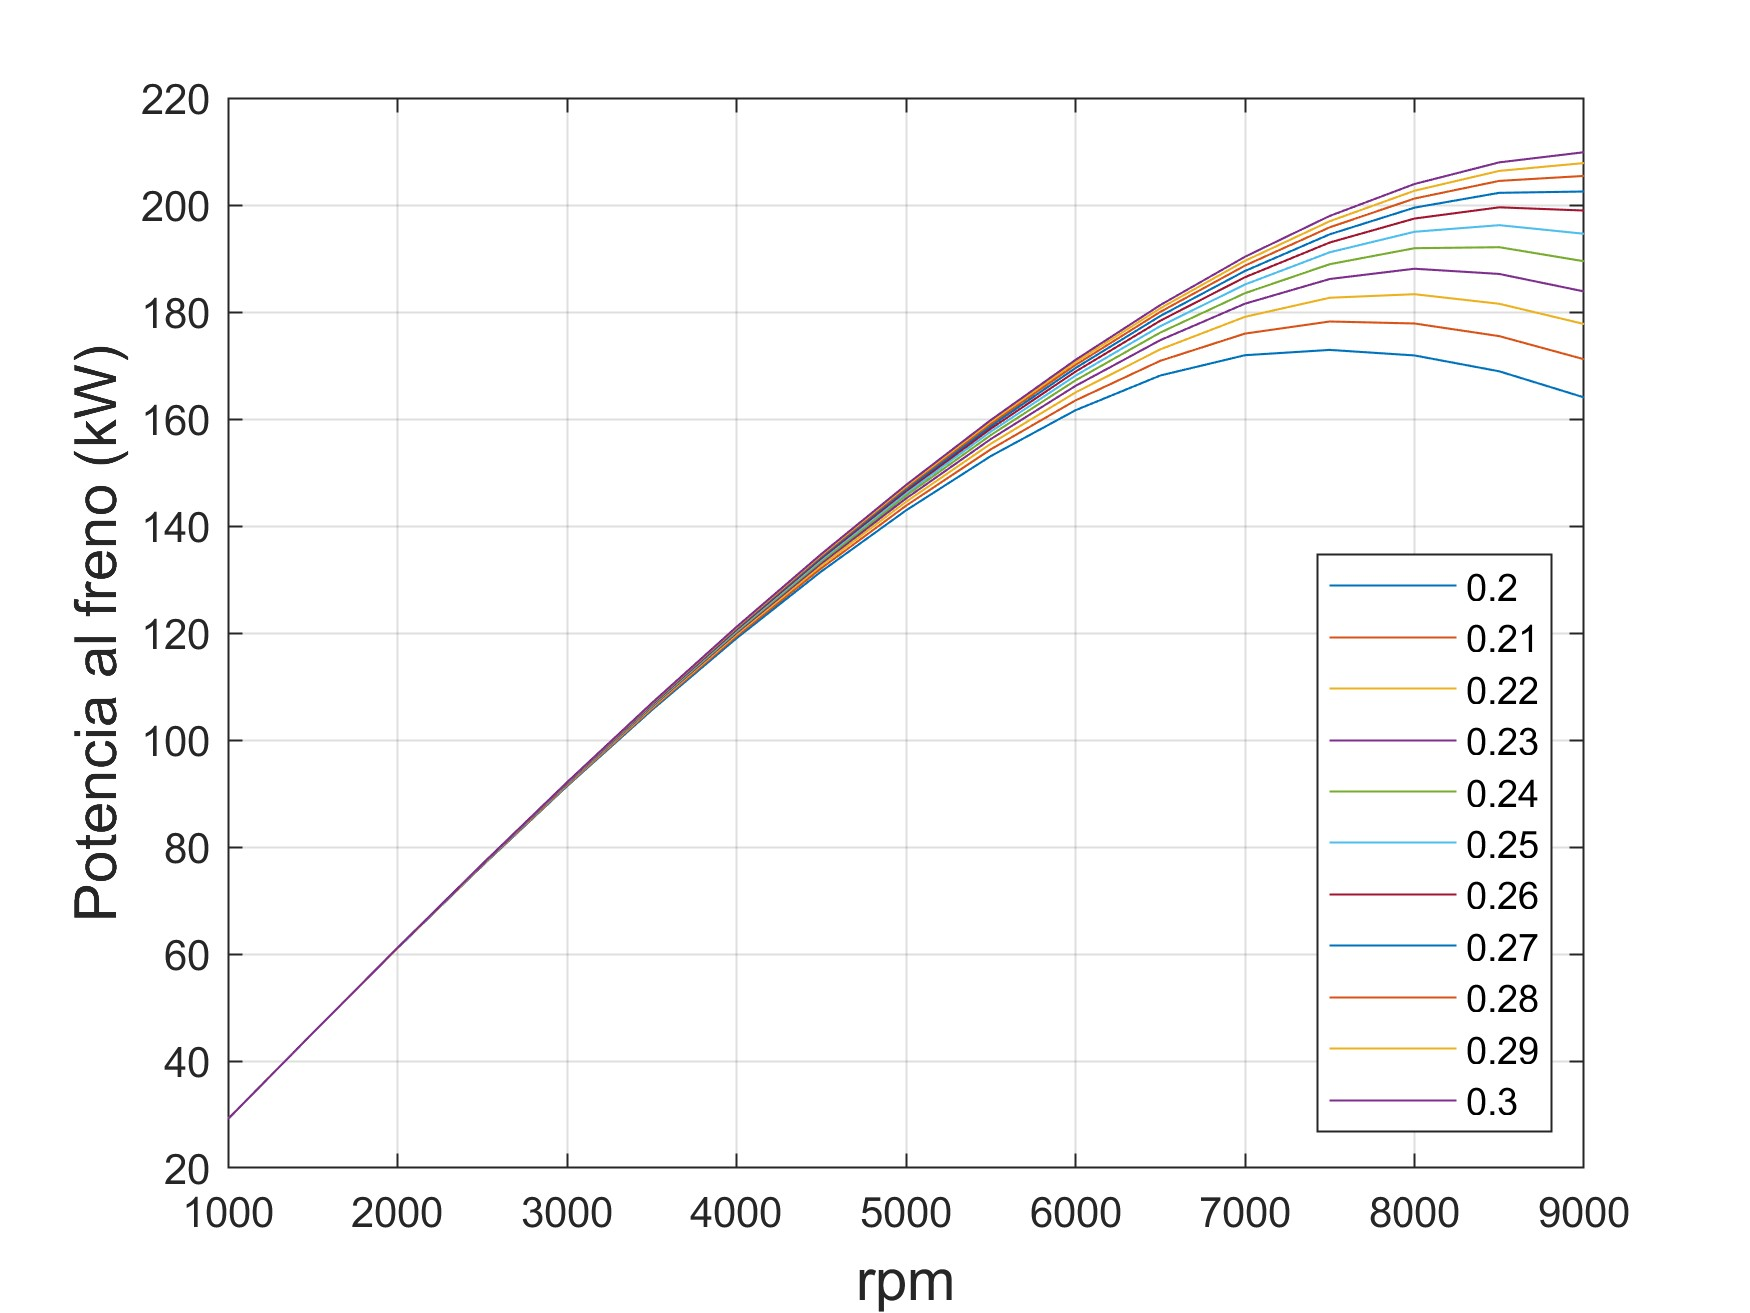
\includegraphics[width=\linewidth]{Figures/01/Potencia_rpm_aval_escape.jpg}
        \caption{Potencia en función de las rpm para dicha área de válvula de escape (AE).}
        \label{fig:RPM_aval_escape}
    \end{subfigure}
    
    % Título principal
    \caption{Potencia en función de las rpm para áreas de válvula de admisión (AA) y de escape (AE).}
    \label{fig:RPM_aval_combined}
\end{figure}

Como era de esperar, se comprueba que un aumento en el tamaño de las válvulas implica un aumento en el flujo de aire que entra al motor y, por tanto, en la potencia producida por el mismo. Sin embargo, existe una limitación geométrica y de propiedades del material a la hora de ir aumentando el tamaño de los agujeros practicados a la culata para alojar dichas válvulas. Por tanto, se tomaron los siguientes valores:

\begin{itemize}
   \item \textbf{Área de válvula de admisión (AA):} 40\%  del área del cilindro.
  \item \textbf{Área de válvula de escape (AE):} 30\%  del área del cilindro.
  \end{itemize}
  

\subsection{Curva de Avance de Encendido} \label{s:subsection_03}

Para determinar la curva de avance de encendido a plena carga del motor se ejecutó un bucle de código que recorre los puntos de funcionamiento a plena carga (presión de soplado del turbo 2.1 bar), con un paso de $50 \ rpm$, y un barrido desde $-20º$ a $40º$ de adelanto de encendido frente al punto muerto superior del tiempo de compresión (siendo valores negativos de AICB retardos), mientras que se guarda en un vector el peligro de detonación para cada una de las combinaciones. Se escoge, entonces, para cada valor de $rpm$, el valor de AICB que más próximo se quede, por debajo, a un peligro de detonación de $1.05$. Mediante esos datos se genera un polinomio de grado 6 que aproxime a la función discreta. Dicho polinomio es la curva analítica que se utiliza para calcular el avance de encendido óptimo a cada régimen de revoluciones.

En la siguiente tabla \ref{tab:rpm_AICB} se presentan algunos de los adelantos de inicio de combustión que evitan la detonación.
\begin{table}[htbp]
    \centering
    \begin{tabular}{|c|c|c|c|c|c|c|c|c|c|}
        \hline
        \textbf{rpm}       & 1000 & 1500 & 2000 & 2500 & 3000 & 3500 & 4000 & 4500 & 5000 \\ 
        \hline
        \textbf{AICB [º]} & -16  & -8   & -2   & 2    & 4    & 6    & 8    & 10   & 10   \\ 
        \hline
        \textbf{rpm}       & 5500 & 6000 & 6500 & 7000 & 7500 & 8000 & 8500 & 9000 & \\ 
        \hline
        \textbf{AICB [º]} & 12   & 14   & 14   & 14   & 16   & 16   & 18   & 18    & \\ 
        \hline
    \end{tabular}
    \caption{Adelantos de inicio de combustión que evitan la detonación en función de las rpm.}
    \label{tab:rpm_AICB}
\end{table}

\begin{figure}[H]
    \centering
    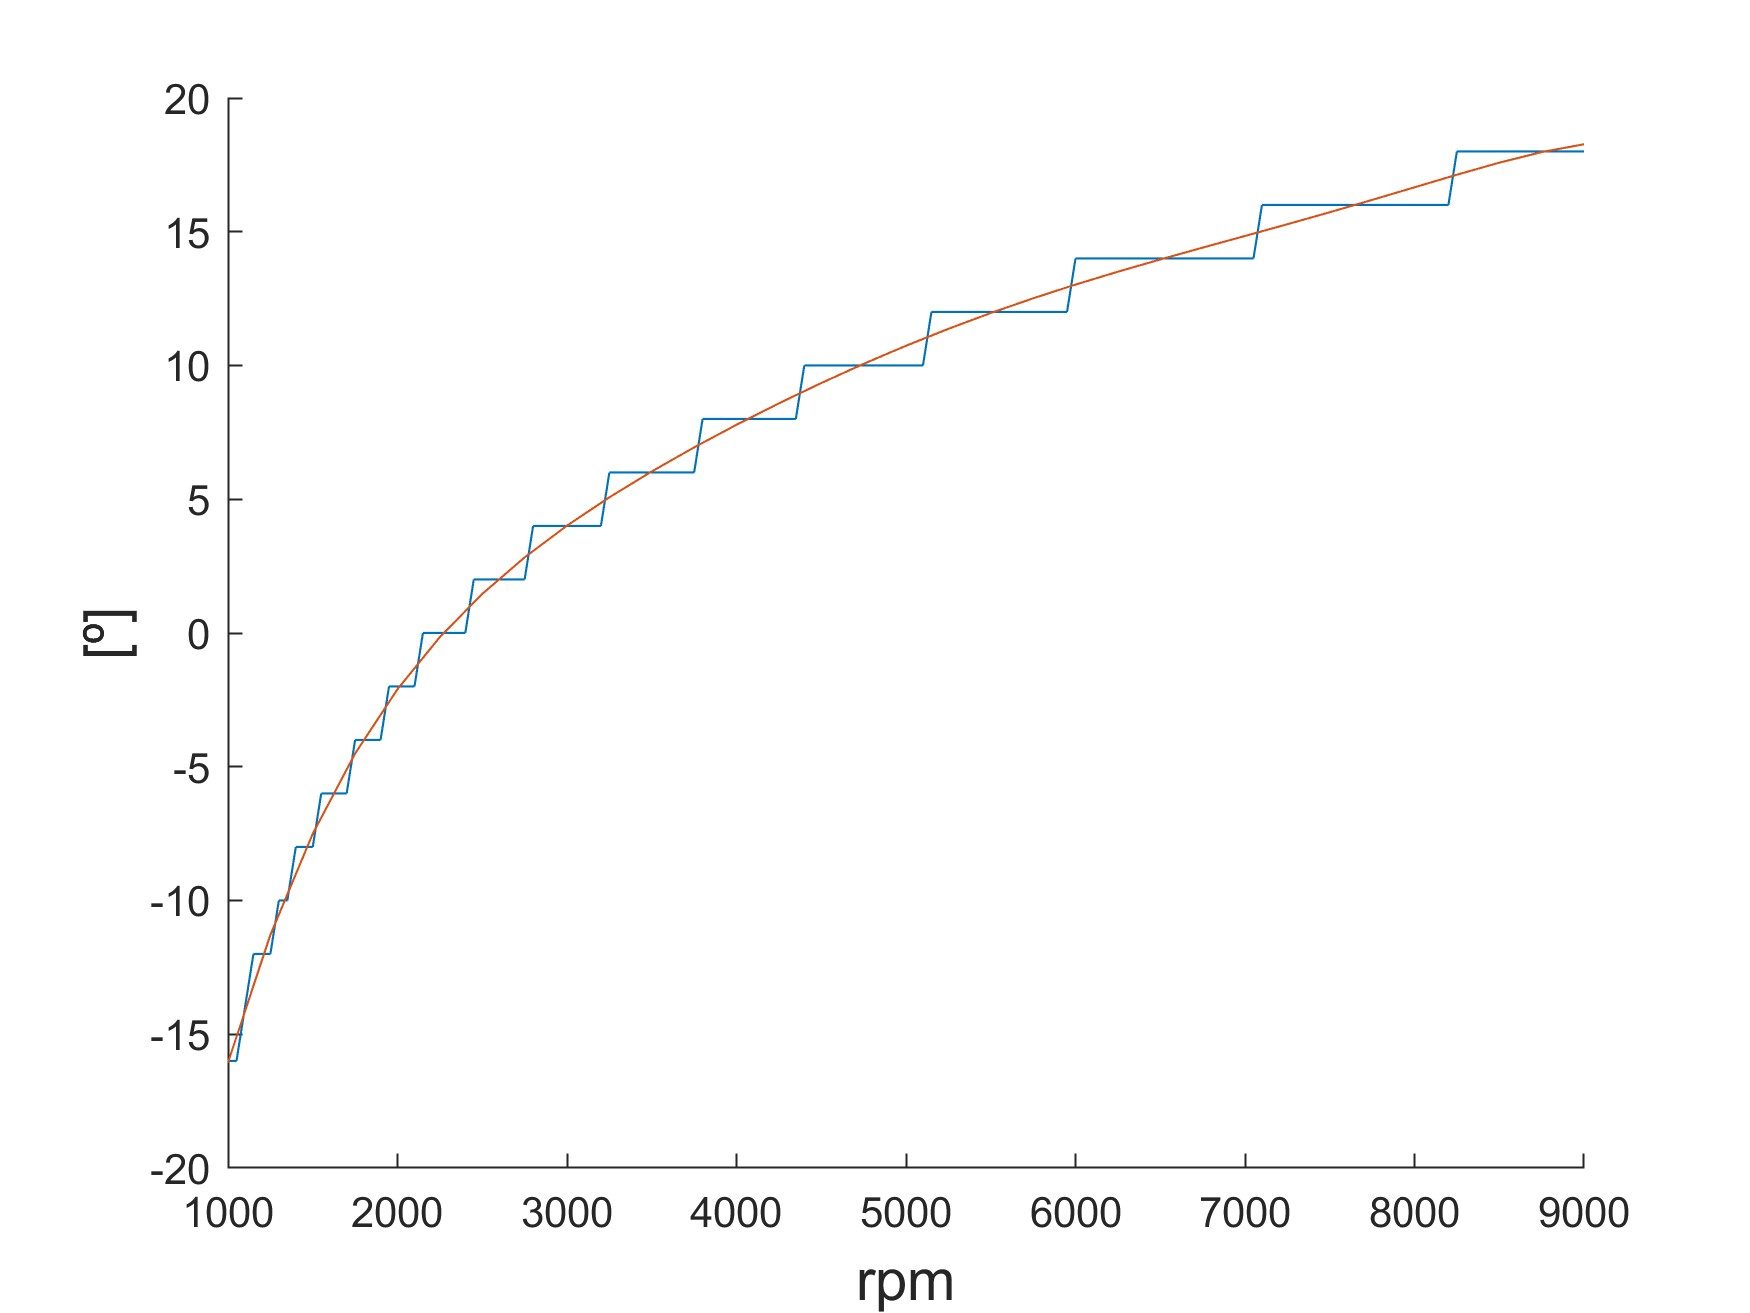
\includegraphics[width=0.6\linewidth]{Figures/01/regresion_aicb.jpg}
    \caption{Adelantos de inicio de conbustión que evitan la detonación en función de las rpm.}
    \label{fig:RPM_aicb}
\end{figure}

\section{Actuaciones del motor} \label{s:section_06}
Con las siguientes tablas y gráficas y mediante una regresión de la que se obtiene un polinomio de tercer grado se obtiene la curva de los retardos al cierre de admisión y adelantos a la apertura de escape que maximizan la potencia en función de las revoluciones por minuto (\textit{rpm}).

\begin{figure}[H]
    \centering
    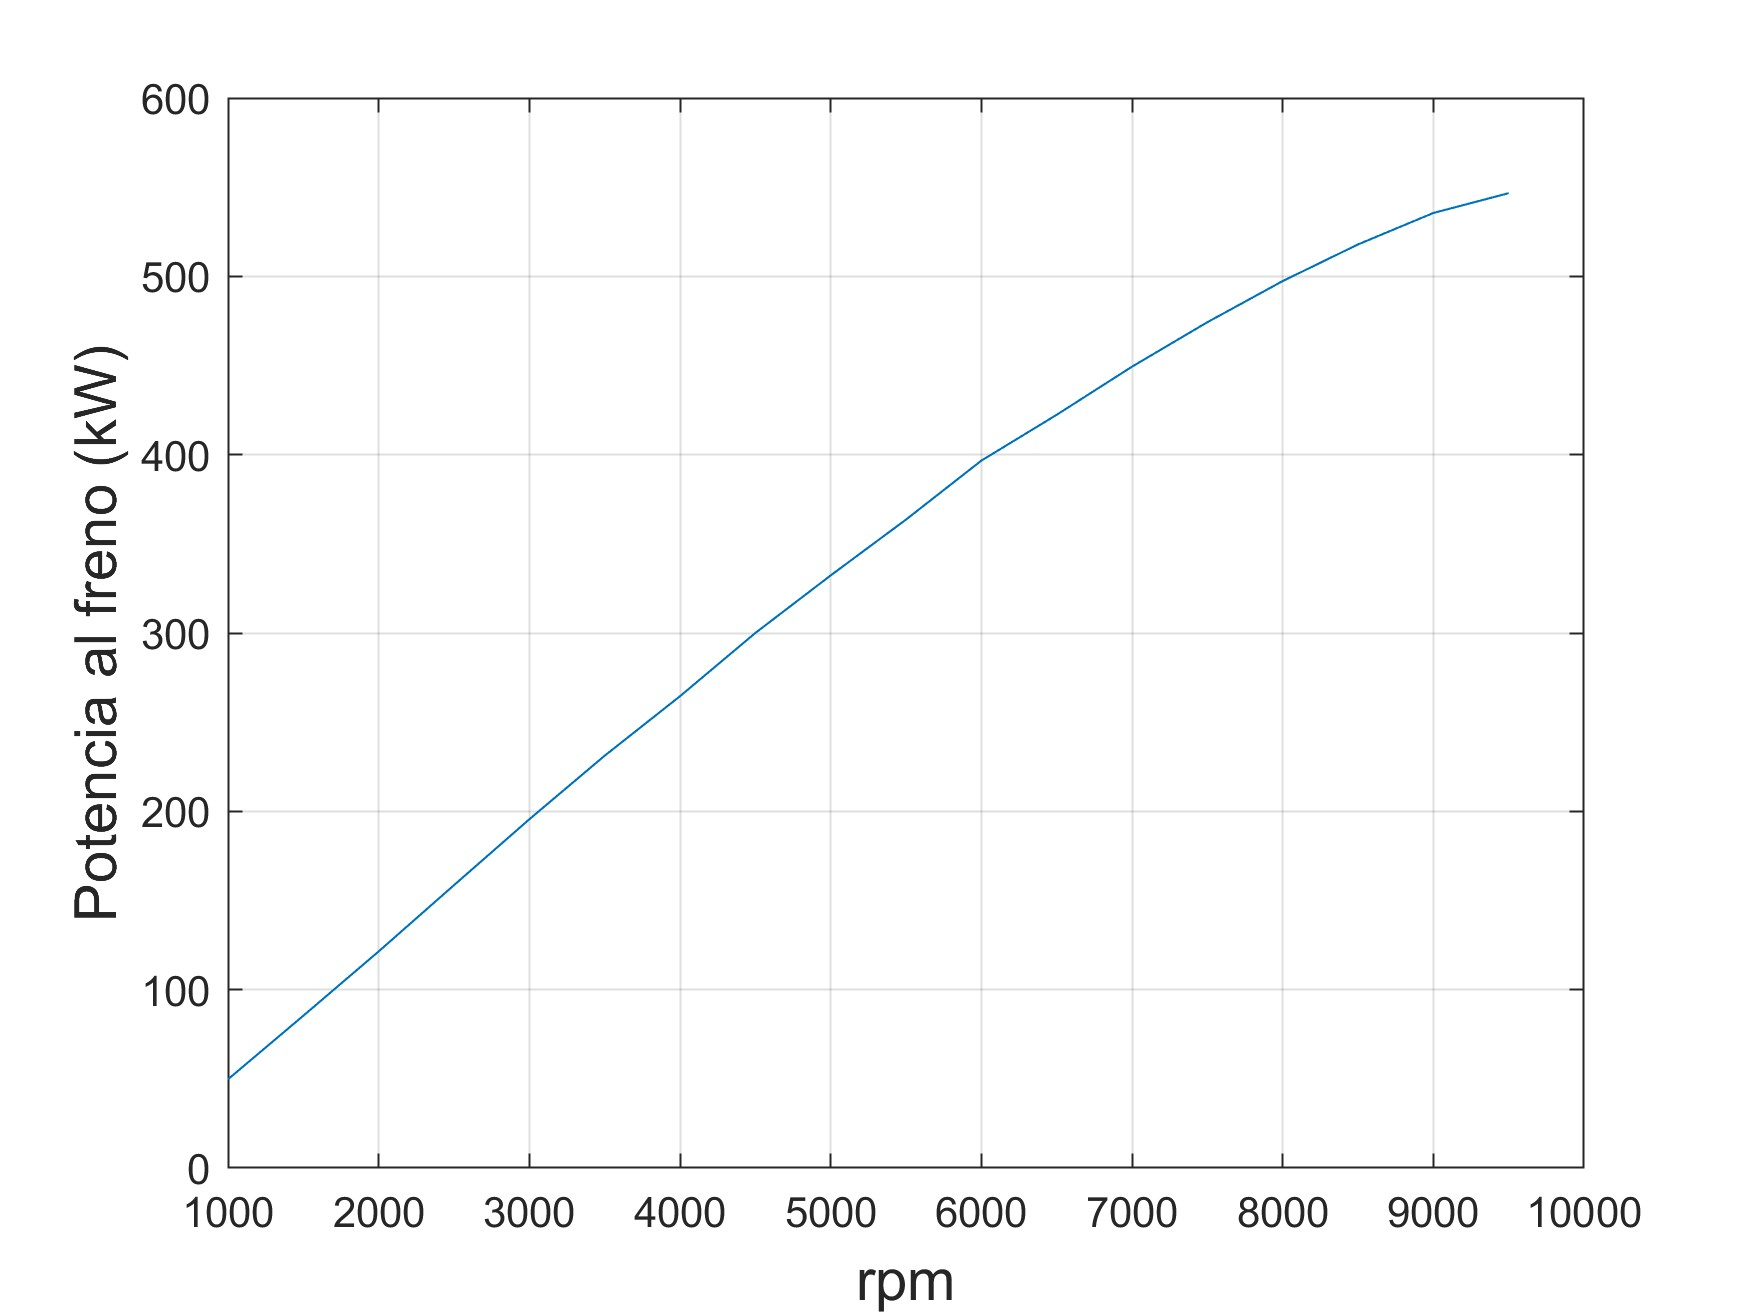
\includegraphics[width=0.6\linewidth]{Figures/01/Potencia_rpm.jpg}
    \caption{Potencia al freno en función de las rpm.}
    \label{fig:RPM_pot}
\end{figure}

\begin{figure}[H]
    \centering
    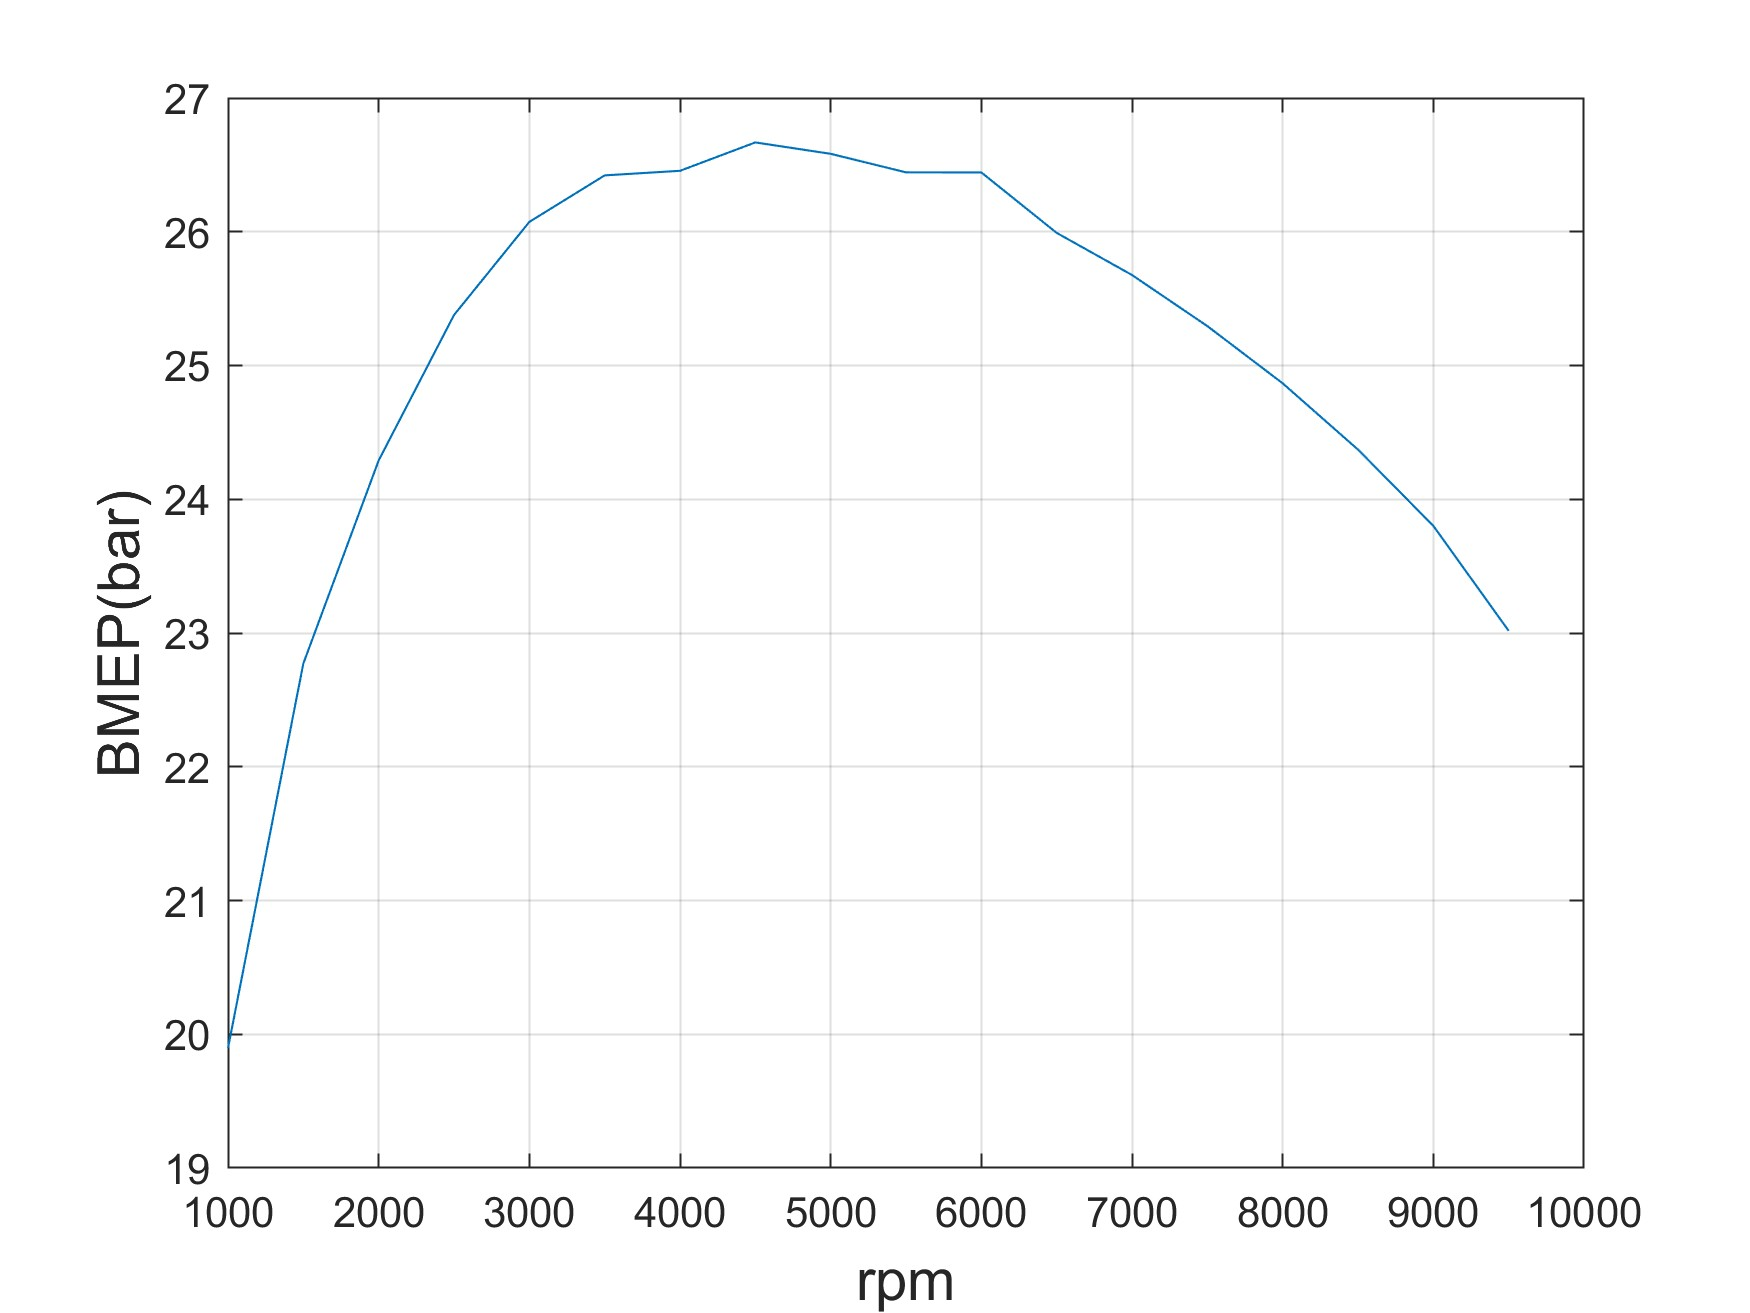
\includegraphics[width=0.6\linewidth]{Figures/01/BMEP.jpg}
    \caption{Presión media efectiva al freno en función de las rpm.}
    \label{fig:RPM_bmep}
\end{figure}


\clearpage


%   ---   BIBLIOGRAFÍA/REFERENCIAS   ---   %

\phantomsection
\addcontentsline{toc}{section}{Referencias}
\renewcommand{\refname}{Referencias}
\bibliographystyle{elsarticle-num}
\bibliography{references.bib}
\clearpage



\end{document}